\section{Testing Calpy}
To ensure everything in calpy acted as expected, tests were run to ensure correctness. This includes testing the detection and measurement of pauses in synthetic monologue, and actual dialogue conversation audio files through the Calpy system. The file frequency formats, filetypes, background noise and entropy systems were also tested.\\


\underline{\textsc{Parameters:}} Min Pause used was 0.001 seconds. Specifically with the function dsp.pause\_profile(sound, fs, 0.001) #pauses counted in units of 1ms

\underline{\textsc{Environment:}} For these test experiments recordings were done by the author in a closed room with no external noise to document the capabilities of the dsp.pause\_processing function in calpy and how well it performed. 


%%%%%%%%%%
% TESTING PAUSE DETECTION
%%%%%%%%%%
\subsection{Test 1: Testing Pause Detection}
\subsubsection{\underline{Test 1.1: Four controlled pauses}}
\begin{description}
	\item[Test:] The test aimed to see at what level calpy could identify each pause. 
				An utterance was recorded by the author and copied three times to produce four pauses in total.
				The pauses were 1s, 10ms, 1ms and 3s respectively.
				The 1ms pause is marked by the black line in the soundwave, otherwise it's too small to be seen.
	\item[File:] The file used was data/pause\_test/500ms\_40ms\_1ms\_3s/ \\
	\space\space\space\space 44100/500ms\_40ms\_1ms\_3s\_44100.wav
	\item[Result:] 3 out of 4 pauses were accounted for. The 1ms pause was not detected.
\end{description}
\begin{figure}[h]
	\center
	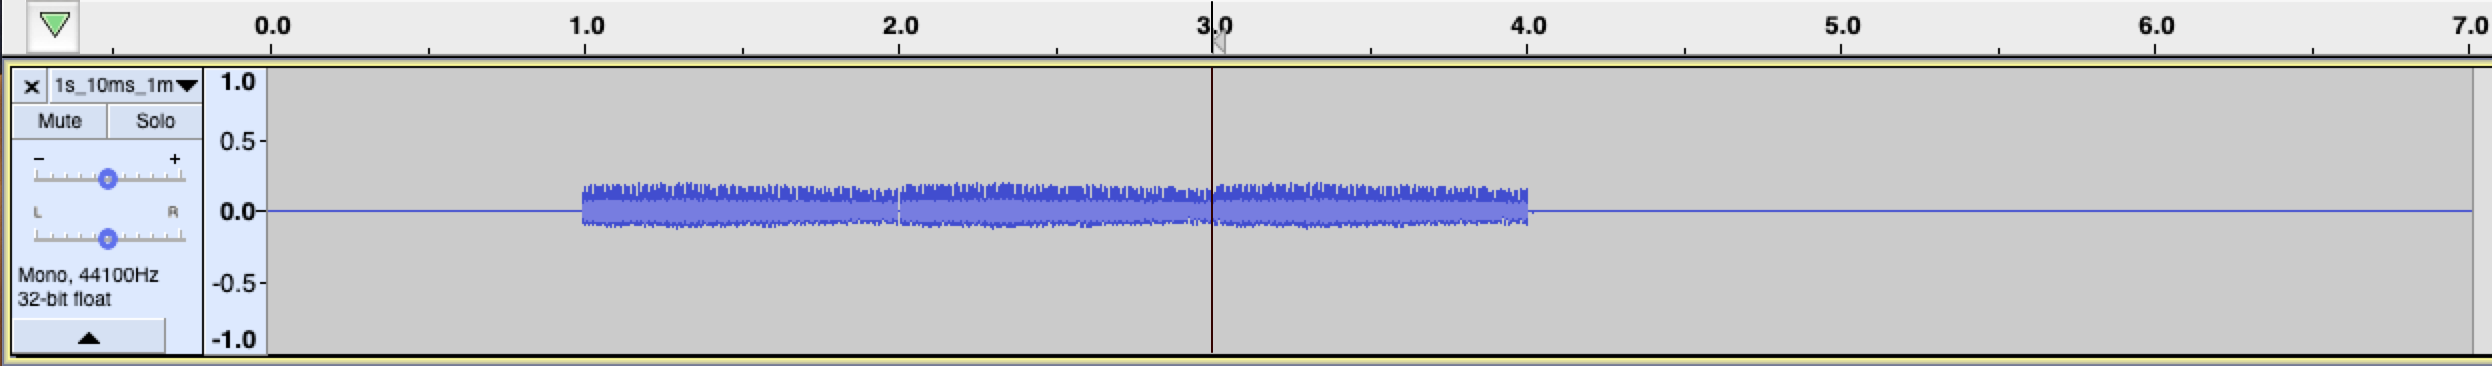
\includegraphics[scale=0.3]{src/main-matter/results/preliminary-testing/detection/1s_10ms_1ms_3s}
	\caption{Waveform of Test 1.1}
	\label{fig:011}
\end{figure}

\subsubsection{\underline{Test 1.2: Counting one to eight}}
\begin{description}
	\item[Test:] The numbers one to eight were counted by the author (very slowly with ample pause) to see where pauses are and aren't detected.
	\item[File:] The file used was data/pause\_test/detection/counting/one\_to\_eight\_robert.wav and can be found in the accompanying data source provided.
	\item[Result:] 9 pauses were accounted for out of a total 9. 
\end{description}
\begin{figure}[h]
	\center
	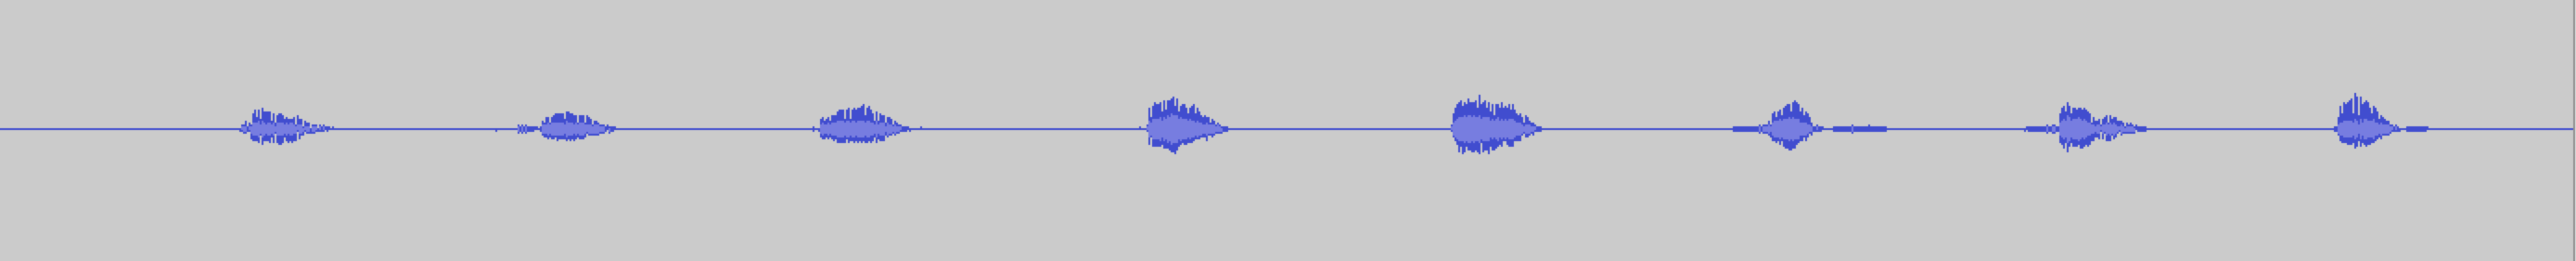
\includegraphics[scale=0.2]{src/main-matter/results/preliminary-testing/detection/011}
	\caption{Waveform of Test 1.2}
	\label{fig:011}
\end{figure}
%
%\paragraph{\underline{Test 1.3: Counting one - Extending initial pause}}
%\begin{description}
%	\item[\underline{Test:}] Seeing where the pause from Test 1.1 is being left out. The audio file from Test 1.1 was taken 
%						and cut down to just the first utterance and surrounding pauses. The initial pause was extended 
%						to help differentiate between the potential returned lengths
%	\item[\underline{File:}] data/pause\_test/detection/counting/one\_robert.wav 
%	\item[\underline{Result:}] A single pause of length 6 was returned
%\end{description}
%\begin{figure}[h]
%	\center
%	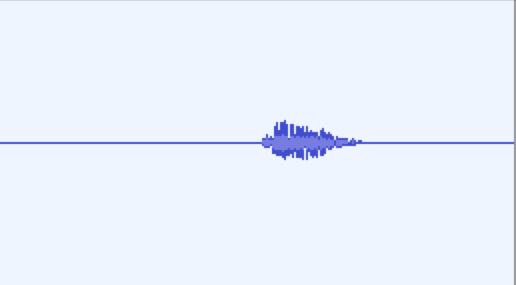
\includegraphics[scale=0.2]{src/main-matter/results/preliminary-testing/detection/012}
%	\caption{}
%	\label{fig:012}
%\end{figure}


%\paragraph{\underline{Test 1.3: Counting one - Extending final pause}}
%\begin{description}
%	\item[\underline{Test:}] The audio from Test 1.2 was used with the final pause extended out
%	\item[\underline{File:}] data/pause\_test/detection/counting/one\_long\_end\_padding\_robert.wav
%	\item[\underline{Result:}] A single pause of length 6 was returned 
%\end{description}
%\begin{figure}[h]
%	\center
%	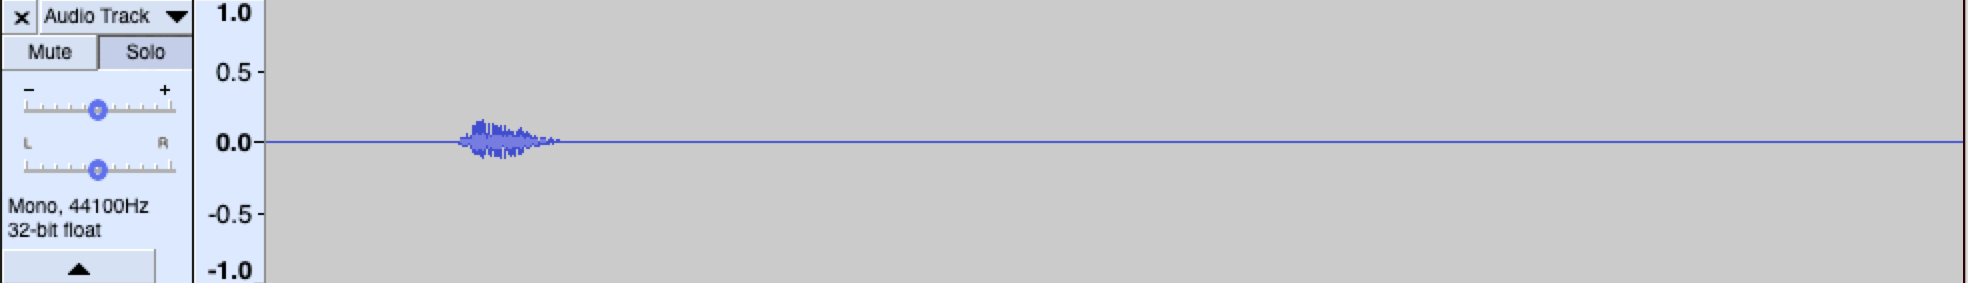
\includegraphics[scale=0.2]{src/main-matter/results/preliminary-testing/detection/013}
%	\caption{}
%	\label{fig:013}
%\end{figure}


%\paragraph{\underline{Test 1.4: Counting one - Further extending initial pause}}
%\begin{description}
%	\item[\underline{Test:}] The audio from Test 1.2 was used with the initial pause further extended to confirm 
%						only the last pause isn't detected
%	\item[\underline{File:}] data/pause\_test/detection/counting/one\_long\_start\_padding\_robert.wav
%	\item[\underline{Result:}] A pause of length 20 was returned 
%\end{description}
%\begin{figure}[h]
%	\center
%	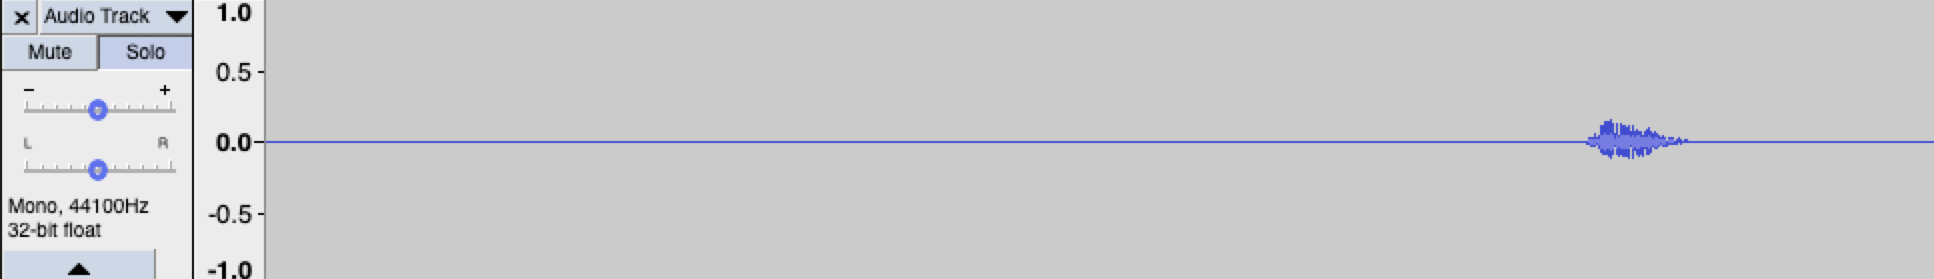
\includegraphics[scale=0.2]{src/main-matter/results/preliminary-testing/detection/014}
%	\caption{}
%	\label{fig:014}
%\end{figure}

\paragraph{\underline{Test 1.3: Counting one to four - Background noise}}
\begin{description}
	\item[Test:] A new audio file was made of the author counting one to four 
				with low background noise of a fan included during recording 
	\item[File:] data/pause\_test/detection/counting/one\_to\_four\_bkg\_fan\_robert.wav
	\item[Result:] 5 pauses returned out of a total 5
\end{description}
\begin{figure}[h]
	\center
	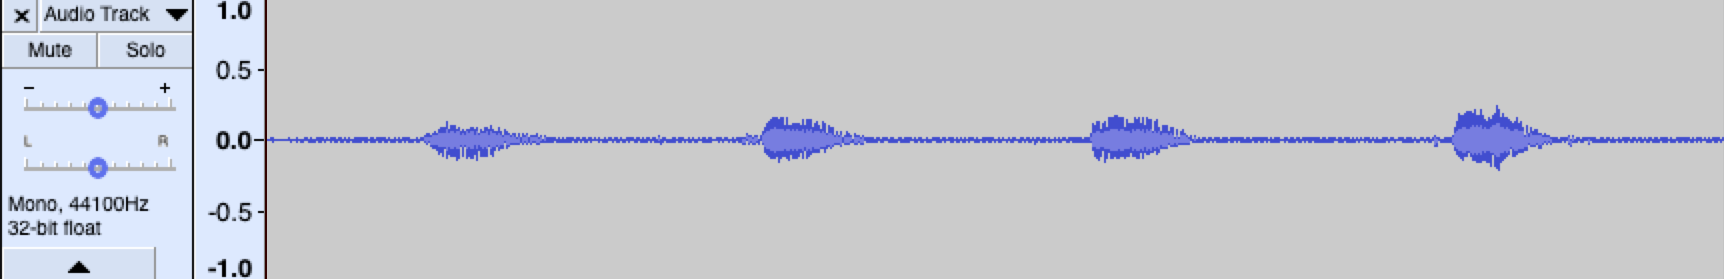
\includegraphics[scale=0.2]{src/main-matter/results/preliminary-testing/detection/015}
	\caption{Waveform of Test 1.3}
	\label{fig:015}
\end{figure}

\paragraph{\underline{Test 1.4: Counting one to five - Background Noise}}
\begin{description}
	\item[Test:] A similar test to test 1.5 with higher intensity background noise 
	\item[File:] data/pause\_test/detection/counting/one\_to\_five\_bkg\_fan\_robert.wav
	\item[Result:] 6 pauses returned out of a total 6
\end{description}
\begin{figure}[h]
	\center
	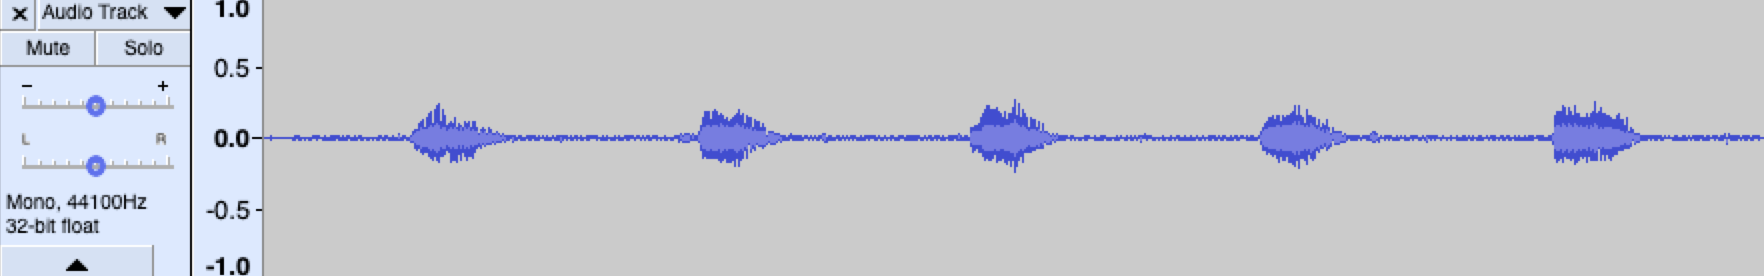
\includegraphics[scale=0.2]{src/main-matter/results/preliminary-testing/detection/016}
	\caption{Waveform of Test 1.4}
	\label{fig:016}
\end{figure}

\paragraph{\underline{Test 1.5: Counting one to six - Relaxed delivery}}
\begin{description}
	\item[Test:] Author counted one to six in a more relaxed speech delivery 
	\item[File:] data/pause\_test/detection/counting/one\_to\_six\_relaxed.wav
	\item[Result:] 7 out of 7 pauses detected. %No pause was detected between the fifth and sixth utterance
\end{description}
\begin{figure}[h]
	\center
	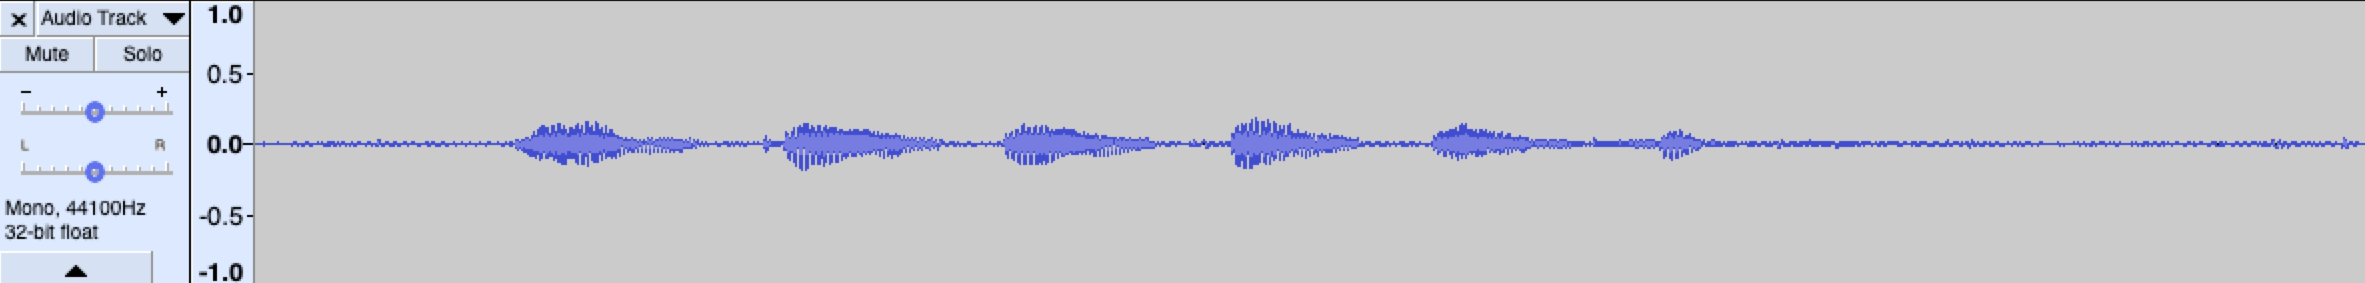
\includegraphics[scale=0.2]{src/main-matter/results/preliminary-testing/detection/017}
	\caption{Waveform of Test 1.5}
	\label{fig:017}
\end{figure}


%\paragraph{\underline{Test 1.8 - Testing Pause Detection - Prose}}
%\begin{description}
%	\item[\underline{Test:}] Author tested in a less controlled speech example by
%						reading a novel for 7 seconds with background noise.  
%	\item[\underline{File:}] data/pause\_test/detection/prose/catch22\_pg1\_7sec.wav
% 	\item[\underline{Output:}]
%	\item[\underline{Result:}] 7 pauses detected out of a total 11 that were intended. 
%%						Of the 9, 2 were pauses less than 1 ms. 
%						Wave form is less distinct as to where pauses are in the audio and shows a 
%						much smoother rise and fall. 
%%						Already this shows a potential breakdown in pause detection. 
%						Results: From the experiment shows micro pause detection doesn't affect the outcome. 
%						This is important because we are not only looking for higher level pauses but also pauses 
%						between words and sentences. 
%\end{description}
%\begin{figure}[h]
%	\center
%	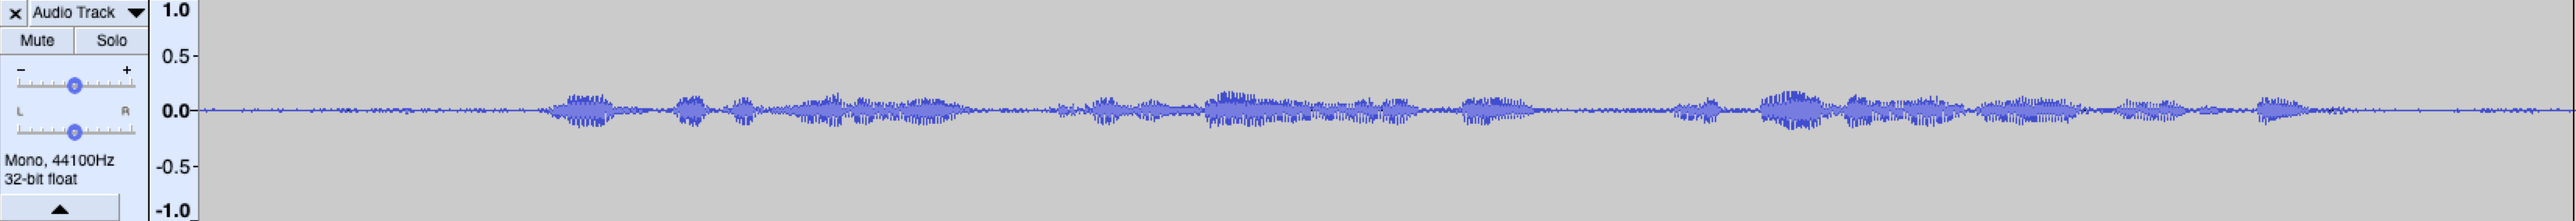
\includegraphics[scale=0.2]{src/main-matter/results/preliminary-testing/detection/018}
%	\caption{}
%	\label{fig:018}
%\end{figure}


\newpage
%%%%%%%%%%
% TESTING PAUSE MEASUREMENT
%%%%%%%%%%
\subsection{Test 2: Testing Pause Length Measurement}
These tests were done to determine how accurate the pause length measurements were. 
%Millisecond was chosen as the time frame because it provided a sufficient level of detail for the experiments. 
%Although finer grain detail would be good, this was all that was required for this thesis.

\paragraph{\underline{Test 2.1: Four Constructed Pauses - [1s, 10ms, 1ms, 3s]}}
\begin{description}
	\item[\underline{Test:}] This test aimed to see how well calpy detects different granularities of pauses. 
						The same audio from test 1.1 was used, the pauses were 1s, 10ms, 1ms and 3s respectively.
						The same utterance is used throughout the recording.
	\item[\underline{File:}] data/pause\_test/timing/nine\_constructed\_pauses.wav
	\item[\underline{Result:}] The output was 10, 1, 30. Indicating calpy is digitising pauses only down to the 100ms level, 
						but still recognising a pause is present (e.g. the 10ms pause still being recognised).
\end{description}
\begin{figure}[h]
	\center
	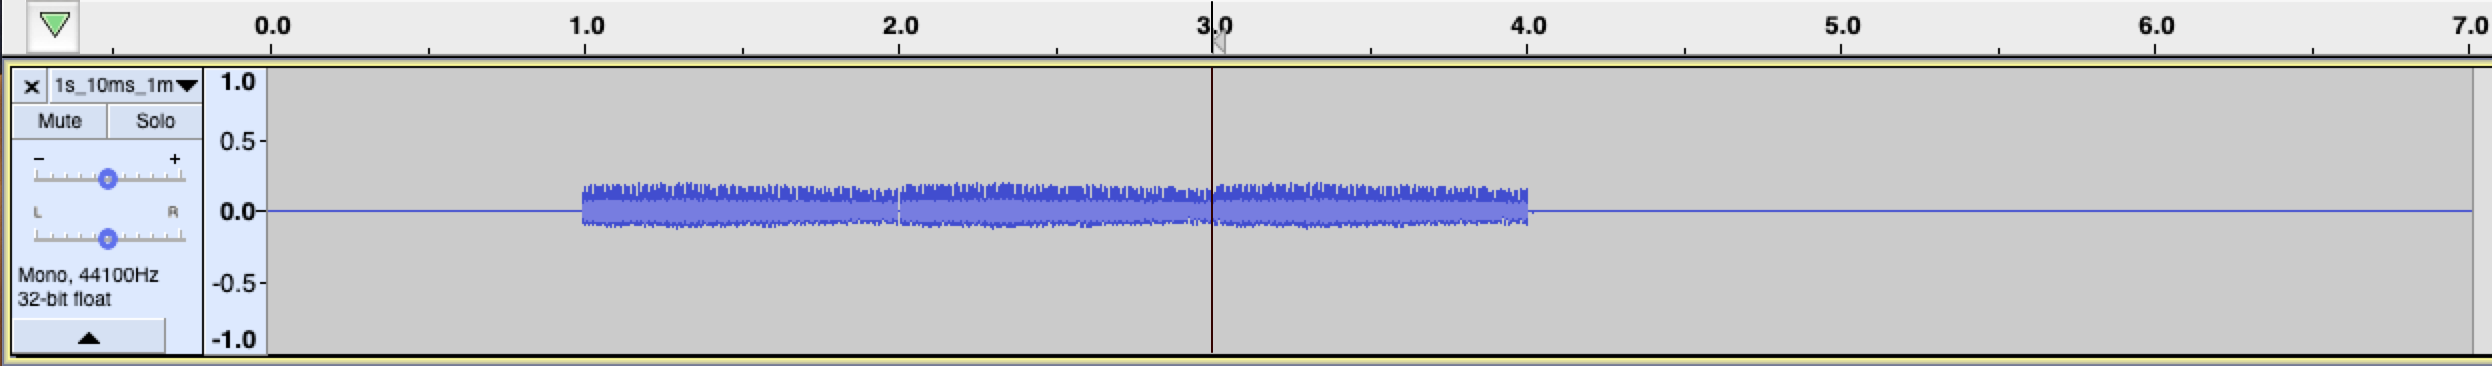
\includegraphics[scale=0.3]{src/main-matter/results/preliminary-testing/detection/1s_10ms_1ms_3s}
	\caption{Four Constructed Pauses of [1s, 10ms, 1ms, 3s]}
	\label{fig:021}
\end{figure}



\paragraph{\underline{Test 2.2: Four Constructed Pauses - [1s, 20ms, 1ms, 3s]}}
\begin{description}
	\item[\underline{Test:}] This test aimed to confirm the digitisation from test 2.1 was correct 
						The same audio from test 2.1 was used, except the 10ms pause was extended to 20ms.
	\item[\underline{File:}] data/pause\_test/timing/nine\_constructed\_pauses.wav
	\item[\underline{Result:}] The output was 10, 1, 30.
\end{description}
\begin{figure}[h]
	\center
	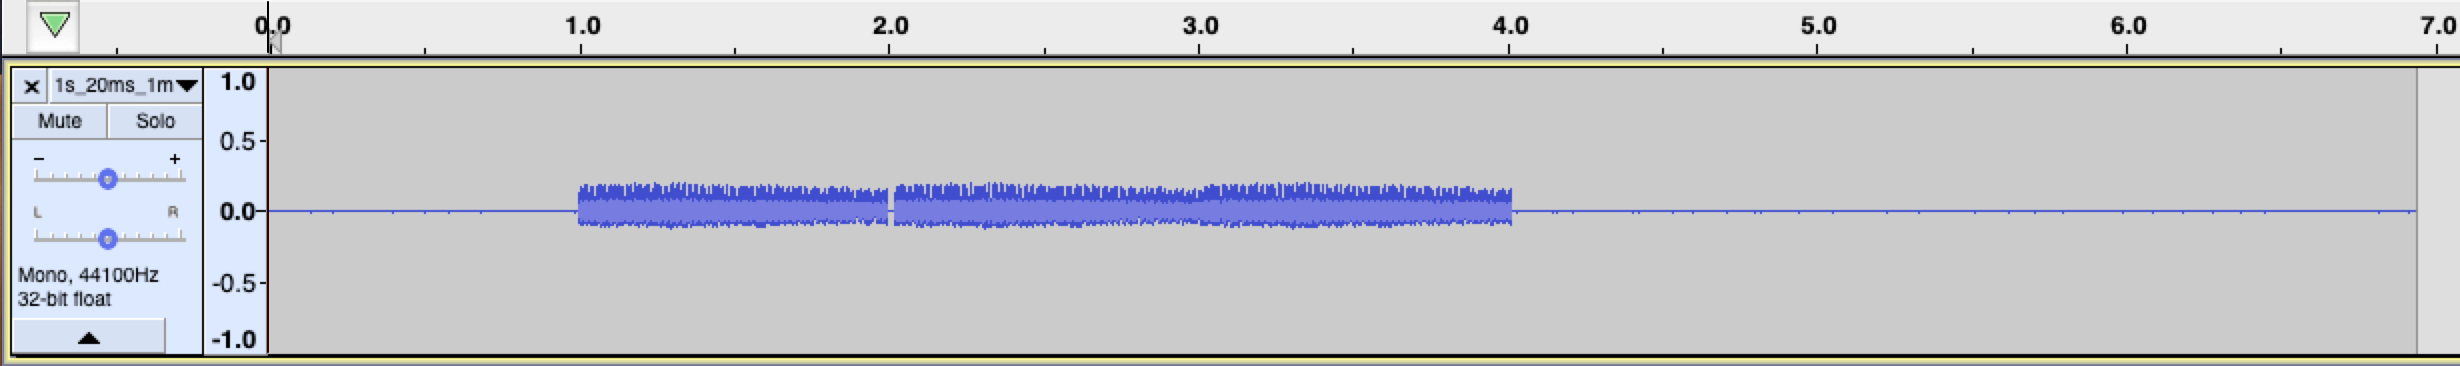
\includegraphics[scale=0.3]{src/main-matter/results/preliminary-testing/detection/1s_20ms_1ms_3s}
	\caption{Four Constructed Pauses - [1s, 20ms, 1ms, 3s]}
	\label{fig:022}
\end{figure}


\paragraph{\underline{Test 2.3: Four Constructed Pauses - [500ms, 40ms, 1ms, 3s]}}
\begin{description}
	\item[\underline{Test:}] This test aimed to further test the digitisation values returned.
						The same audio from test 2.2 was used, except the 20ms pause was extended to 40ms
						and the 1s pause was reduced to 500ms.
	\item[\underline{File:}] data/pause\_test/timing/nine\_constructed\_pauses.wav
	\item[\underline{Result:}] The output was 5, 1, 30.
\end{description}
\begin{figure}[h]
	\center
	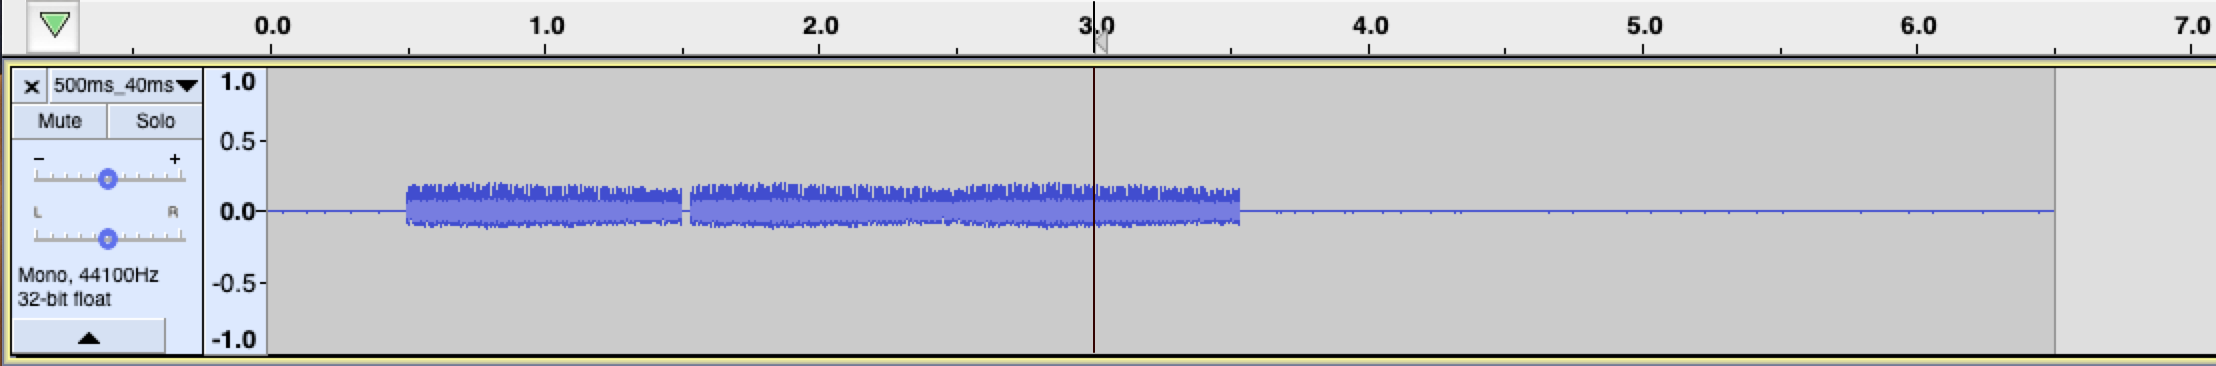
\includegraphics[scale=0.3]{src/main-matter/results/preliminary-testing/detection/500ms_40ms_1ms_3s}
	\caption{Four Constructed Pauses - [500ms, 40ms, 1ms, 3s]}
	\label{fig:023}
\end{figure}


\paragraph{\underline{Test 2.4: Four Constructed Pauses - [500ms, 80ms, 1ms, 3s]}}
\begin{description}
	\item[\underline{Test:}] This test aimed to further test the digitisation values
						The same audio from test 2.3 was used, except the 40ms pause was extended to 80ms.
	\item[\underline{File:}] data/pause\_test/timing/nine\_constructed\_pauses.wav
	\item[\underline{Result:}] The output was 5, 1, 30.
\end{description}
\begin{figure}[h]
	\center
	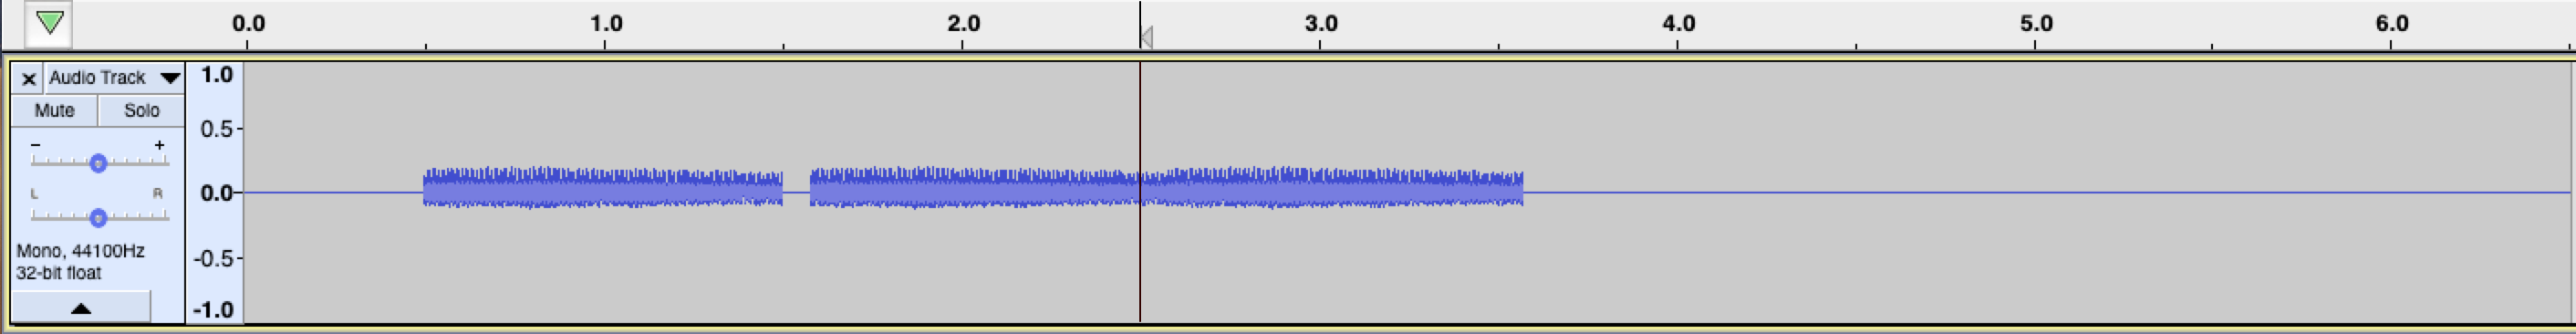
\includegraphics[scale=0.3]{src/main-matter/results/preliminary-testing/detection/500ms_80ms_1ms_3s}
	\caption{Four Constructed Pauses - [500ms, 80ms, 1ms, 3s]}
	\label{fig:023}
\end{figure}

\paragraph{\underline{Test 2.5: Four Constructed Pauses - [500ms, 40ms, 9ms, 3s]}}
\begin{description}
	\item[\underline{Test:}] This test aimed to further test the digitisation values
						The same audio from test 2.3 was used, except the 1ms pause was extended to 9ms.
	\item[\underline{File:}] data/pause\_test/timing/nine\_constructed\_pauses.wav
	\item[\underline{Result:}] The output was 5, 1, 1, 30.
\end{description}
\begin{figure}[h]
	\center
	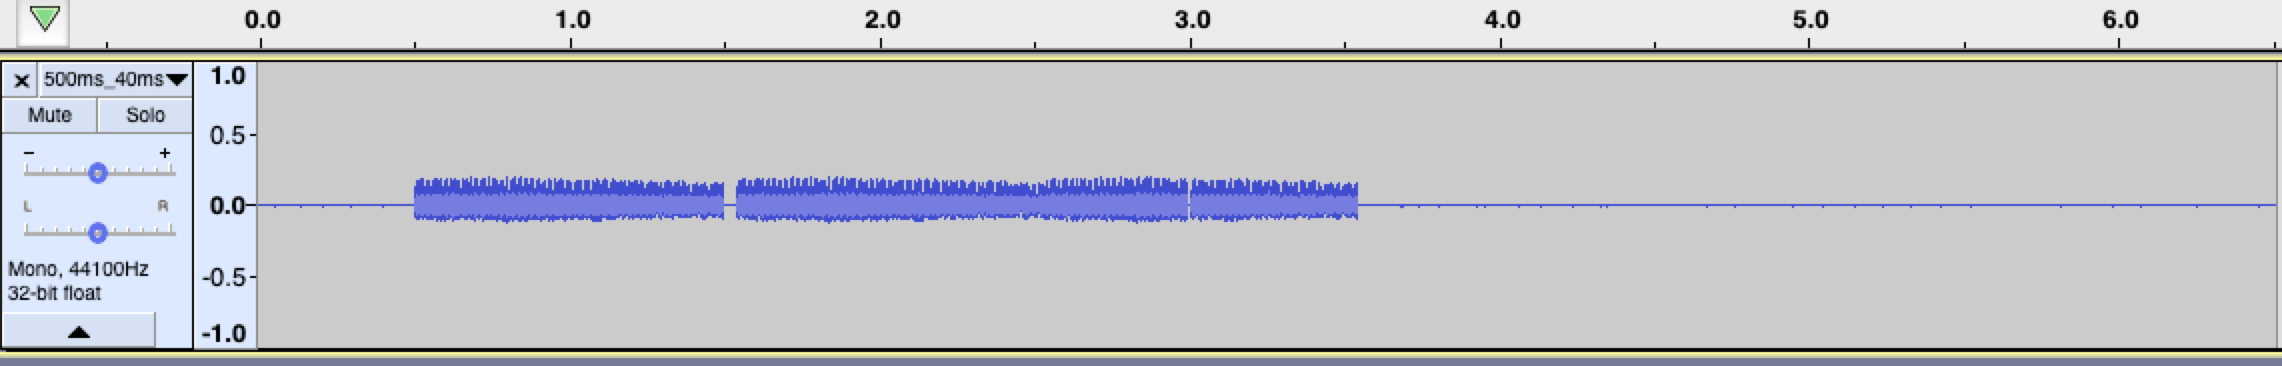
\includegraphics[scale=0.3]{src/main-matter/results/preliminary-testing/detection/500ms_40ms_9ms_3s}
	\caption{Four Constructed Pauses - [500ms, 80ms, 1ms, 3s]}
	\label{fig:023}
\end{figure}

\subsubsection{Test 2 Results}
The results showed that digitisation is done at the 100ms level but that pauses can be detected down at the 9ms level

%%%%%%%%%%%%
%% LENGTHS vs RATES
%%%%%%%%%%
\subsection{Test 3: Pause Lengths vs Sample Rates}


file\_name = '/OSR\_us\_000\_0030\_8k' \\

file\_path = '/monologue/OSR/Male' + file\_name

\begin{figure}[h]
	\center
	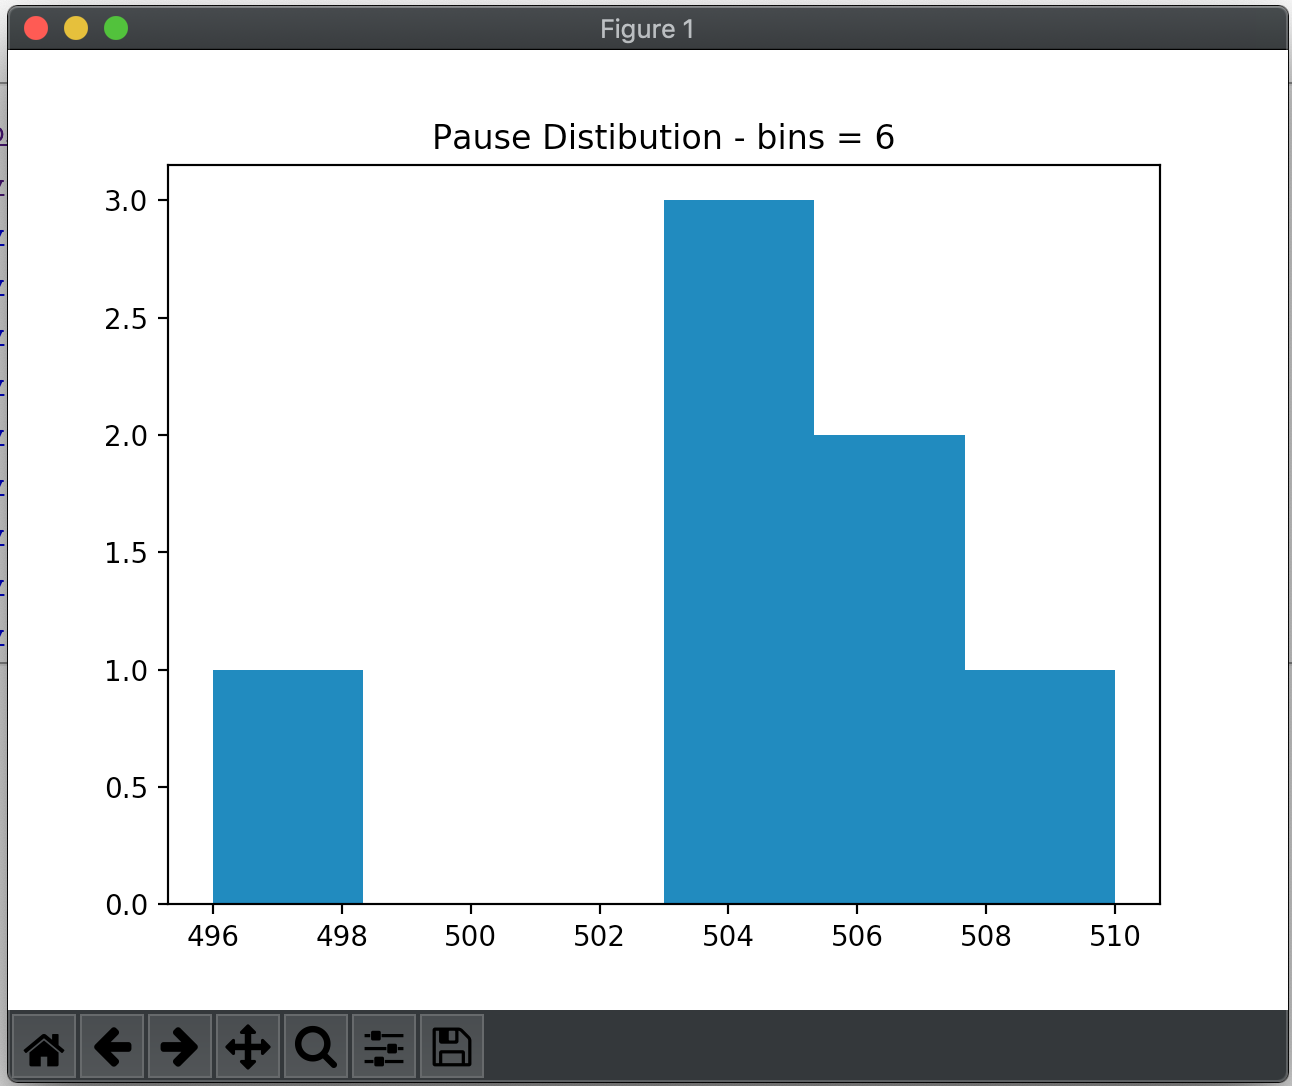
\includegraphics[scale=0.2]{src/main-matter/results/preliminary-testing/sample-rates/031}
	\caption{Sample Rates 1}
	\label{fig:031}
\end{figure}

\begin{figure}[h]
	\center
	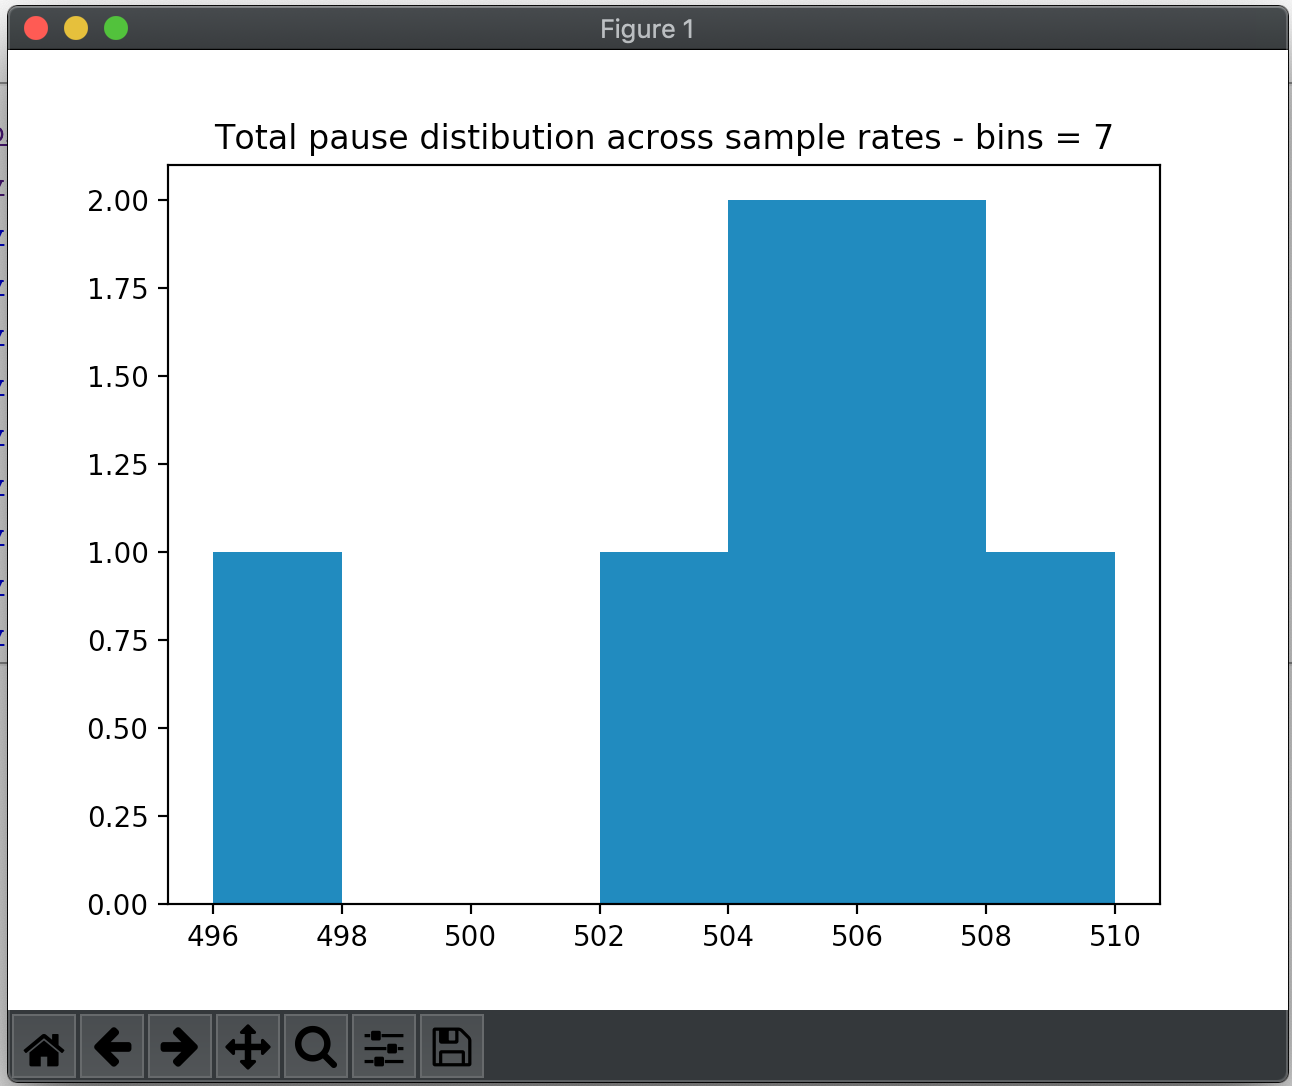
\includegraphics[scale=0.2]{src/main-matter/results/preliminary-testing/sample-rates/032}
	\caption{Sample rates 2}
	\label{fig:032}
\end{figure}

%\subsection{Test 4: Monologue Tests}
This section looks at self recordings and recordings from others online. This was done to increase the variance through different voice types, recording types (freq?)?, different cadences, different recording environments. 

Pauses were counted for some, but more will be done.

\paragraph{Test 4.1:} Grab pauses for a self made audio file (e.g. not from the talk bank)

This is in ideal conditions where the bitrate is high, the pauses are distinct and clear

Remember to Get the pauses checked for correctness once I show I can get a histogram i.e. manually go through and see that pauses are accounted for to show the validity of the algorithm/code 

\paragraph{Test 4.2:} Grab speech audio file from online, test, grab histograms 

\paragraph{Test 4.2.1:} Open Speech Repository (Is this an experiment?)

Reason for Experiment: This was used to show a distinction between the natural conversations taken from E1.2.2 and the more stilted pausing of this recording. 

The downside to this was the pause distribution it produced is of a different conversation type, monologue instead of dialogue. And the audio files are only 30 seconds in length compared to the 30min avg for the talkbank files. So pause frequencies were not as abundant as they would be for longer files. I decided to take the collection of pause frequencies and plot them on a single histogram. I also plotted the change in pause types between male and female speakers. 

- URL to repo
https://www.voiptroubleshooter.com/open\_speech/american.html

Another way to do this would be to grab lectures and see how they compare. They would be much longer and give more detailed pause analysis and I'm sure there a bunch of good quality lecture recordings I could grab to do this on. 

/ca/SCOTUS/OralArguments/ was another that showed multiple single speakers

\subsubsection{Female speaker}
Reason for experiment: 
\paragraph{Test 4.2.1: Lady Speaking 1}
    
Audio file link, Raw pause output
Histogram figure: 

\begin{figure}[h]
    \centering
    \begin{minipage}{0.45\textwidth}
        \centering
        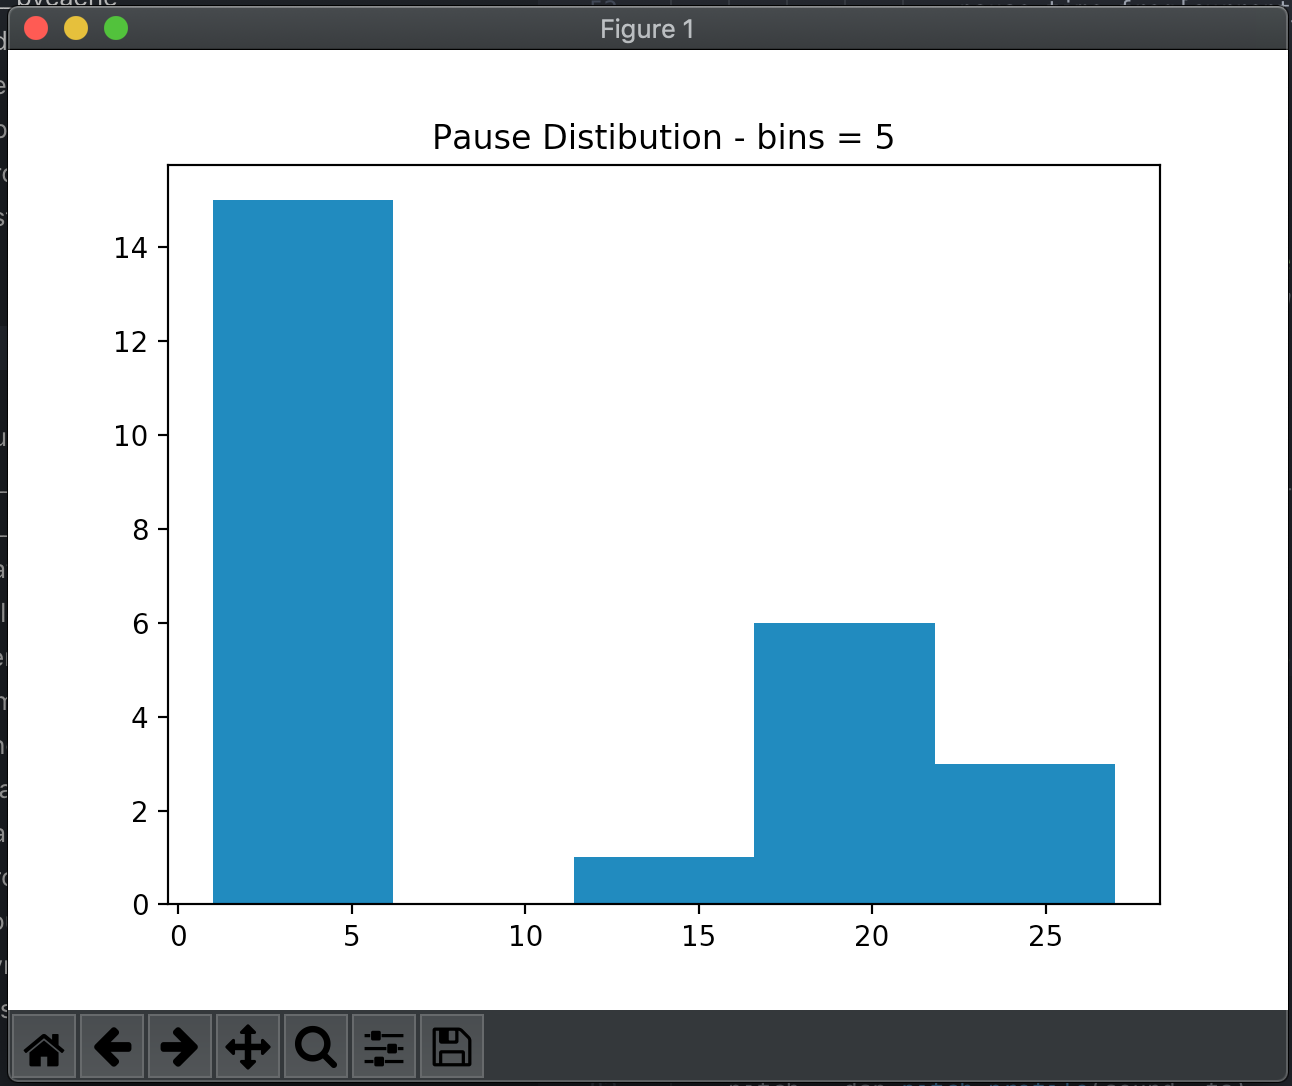
\includegraphics[scale=0.2]{src/main-matter/methodology/pause-distributions/monologue/lady1-1} 
        \caption{Lady Speaking 1-1}
    \end{minipage}\hfill
    \begin{minipage}{0.45\textwidth}
        \centering
        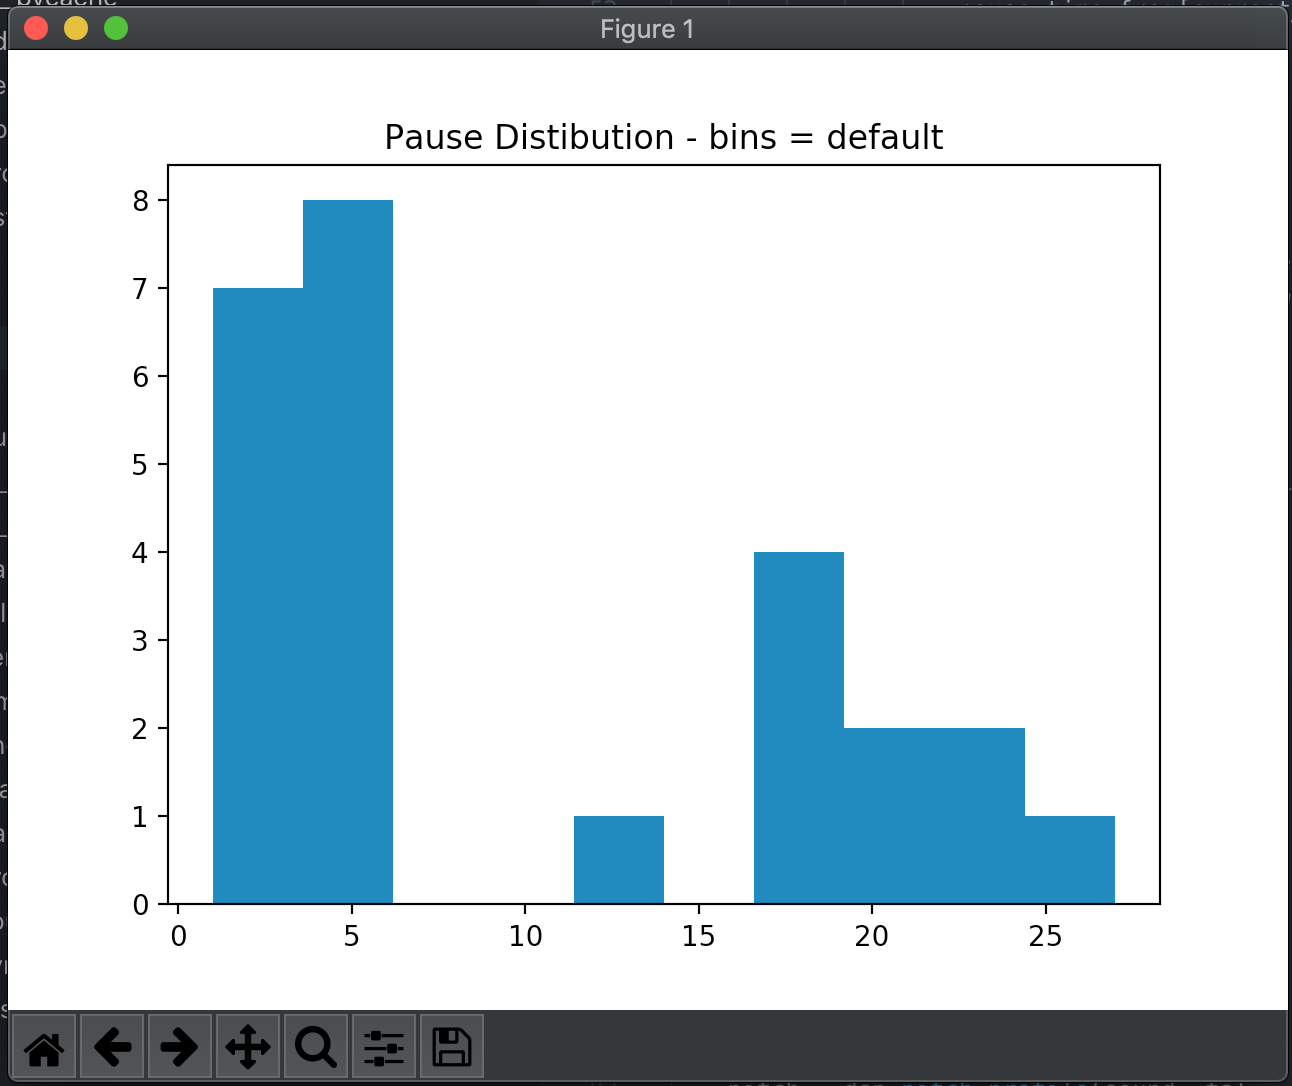
\includegraphics[scale=0.2]{src/main-matter/methodology/pause-distributions/monologue/lady1-2} 
        \caption{Lady Speaking 1-2}
    \end{minipage}\hfill
    \begin{minipage}{0.45\textwidth}
        \centering
        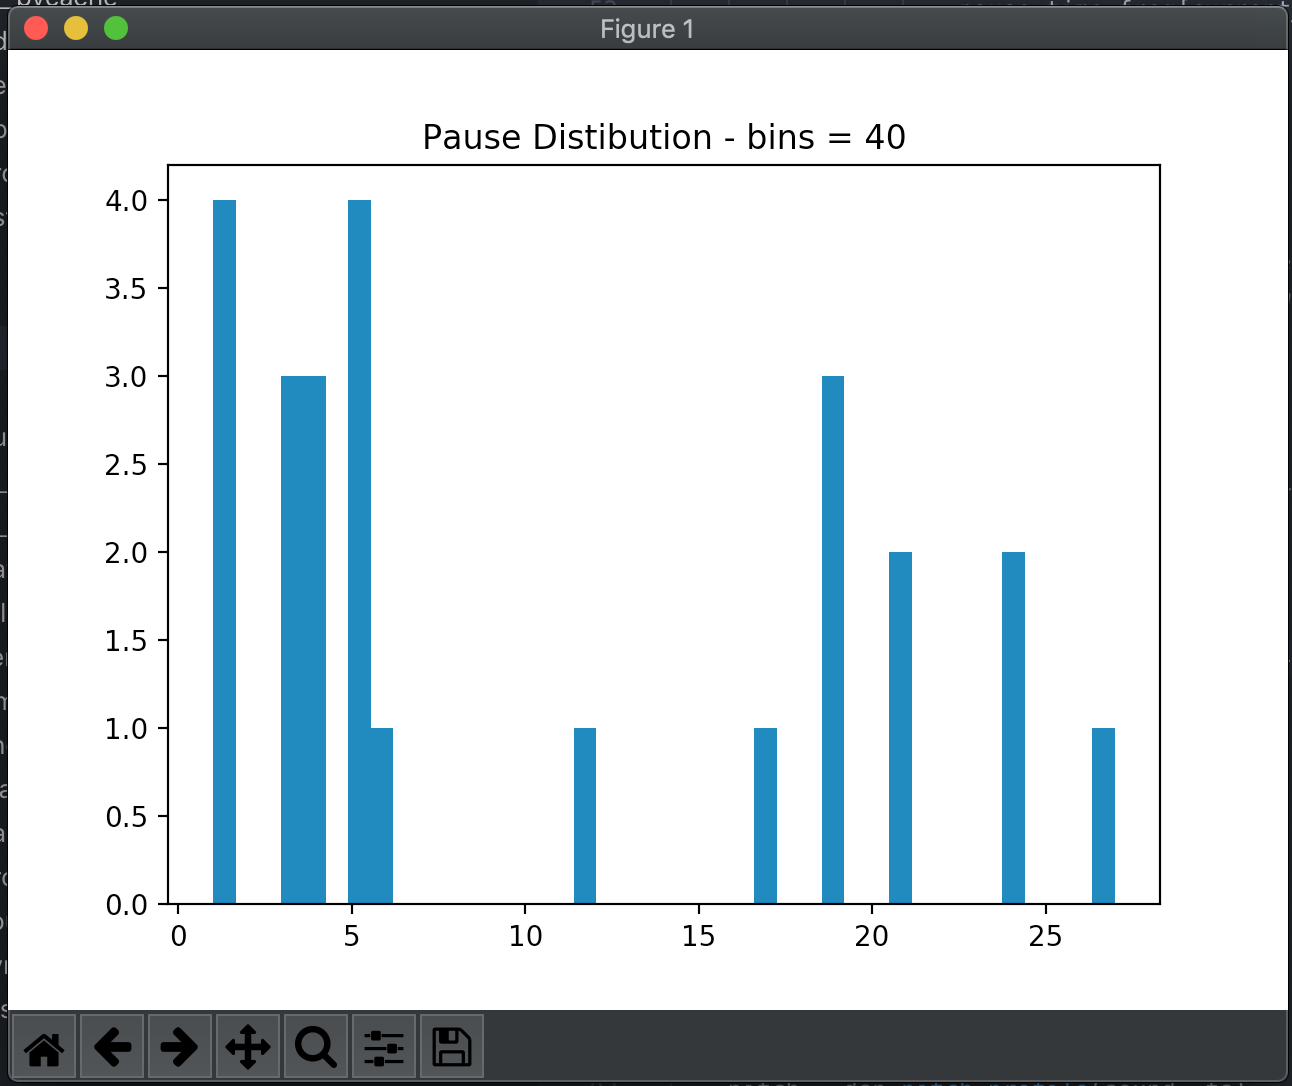
\includegraphics[scale=0.2]{src/main-matter/methodology/pause-distributions/monologue/lady1-3} 
        \caption{Lady Speaking 1-3}
    \end{minipage}
\end{figure}

Findings: Pauses tended to clump together around 0-20ms

\paragraph{Test 4.2.2: Lady Speaking 2}
Link to Audio file, Raw pause output

Histogram
Findings
        
        
        
\subsubsection{Male Speaker}
\paragraph{Test 4.2.3: Man Speaking - 1}
Audio file, Raw pause output can be found at the output\\monologue\\OSR\_us\_000\_0030\_8k directory
Histogram 
\begin{figure}[h]
	\begin{center}
		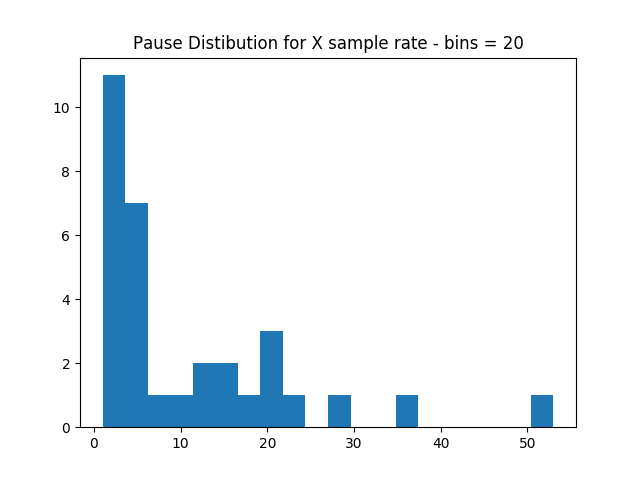
\includegraphics[scale=0.2]{src/main-matter/methodology/pause-distributions/monologue/man1-1}
		\caption{Man Speaking 1-1}
		\label{default}
	\end{center}
\end{figure}
Findings: Pauses tended to clump together around 0-20ms, Should test on wider bin size

\paragraph{Test 4.2.4: Man Speaking 2} 
Link to Audio File, pause output - (OSR\_us\_000\_0061\_8k)
list data output directory location that has everything we need in it
Histogram: 
Findings: Pauses tended to clump around 0-10ms, maybe smaller grained, Needed to test on wider bin 

\paragraph{Test 4.2.5: Man Speaking 3}
\begin{figure}[h]
	\begin{center}
		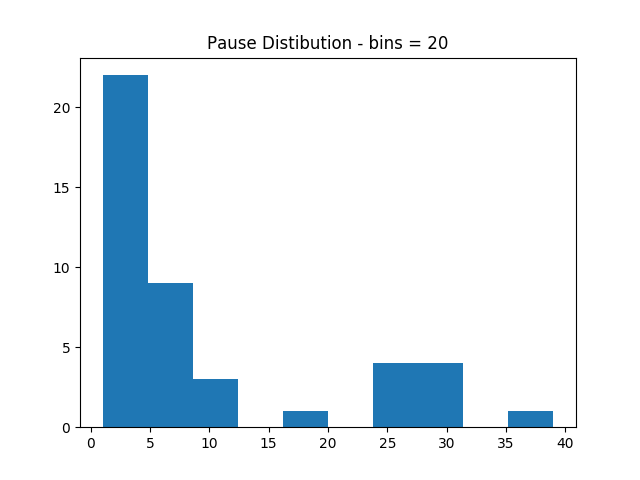
\includegraphics[scale=0.2]{src/main-matter/methodology/pause-distributions/monologue/man2-1}
		\caption{Man Speaking 2-1}
		\label{default}
	\end{center}
\end{figure}
    Findings


\paragraph{Conclusions:} These experiments showed a tendency, even in stilted audio, to tend towards short pauses around the 0-20ms mark. Where the curve tended to be heavily right skewed.

\newpage
\subsection{Test 3: File Format Frequency}
A variety of file frequency formats were tested to see how they differed in terms of pause count and pause measurement. 
This test was done using the talkbank file 6269 as it was the best representative of the talkbank files. 
This was done to understand the impact file format frequency had on resulting pause data.  
%As this takes a long time to compute, only a sample of the data was selected for these tests. Of those files there were preliminary tests were done to see what pause data looked like initially from these and the best and worst performers were chosen to see how they change with frequency change. I think 5000, 4894, 4888, something like that were really bad. Essentially the outliers from these graphs. 


%The digitisation of the audiofile required the most amount of time but increased heavily as audio file size increased. \\

\begin{tabular}{ |p{1.8cm}| |p{1.5cm} |p{1.5cm} |p{1.3cm} |p{1.1cm} |p{1.4cm} |p{1.5cm} |p {1.4cm} |}
	\hline
	\multicolumn{8}{|c|}{CallFriend - English (Northern) - 6269} \\%
	\hline
	{\small Audio File} & 
	{\footnotesize Time taken (min:sec)} & 
	{\footnotesize Binary Pause Array Length} & 
	{\footnotesize Total Audio Pause} & 
	{\footnotesize Total Sounding} & 
	{\footnotesize Pause Proportion} & 
	{\footnotesize Num. of Pauses} & 
	{\footnotesize Avg. Pause Length} \\
		\hline\hline
		%\cellcolor[HTML]{A2A1A2} 
%		8000 & 00:00 & xxxxx & xxxxx & xxx & xx.xx\% & xxx  & xx.xx \\
%		\hline 
		11025 & 02:16 & 18040 & 17367 & 673 & 96.27\% & 507  & 3425ms \\
		\hline 
		\rowcolor{lightgray} 
		16000 & 03:40 & 17999 & 17348 & 651 & 96.38\% & 496 & 3498ms \\
		\hline
		22050 & 04:48 & 18040 & 17362 & 678 & 96.24\% & 510 & 3404ms \\
		\hline
		32000 & 07:01 & 17999 & 17336 & 663 & 96.32\% & 503 & 3447ms \\
		\hline
		44100 & 9:30 & 17999 & 17332 & 667 & 96.30\% & 507 & 3419ms \\
		\hline
		48000& 11:27 & 17999 & 17336 & 663 & 96.32\% & 504 & 3440ms \\
		\hline
		88200 & 13:32 & 17999 & 17333 & 666 & 96.30\% & 503 & 3446ms \\
		\hline
		96000 & 15:42 & 17999 & 17334 & 665 & 96.31\% & 505 & 3432ms \\
		\hline
%		Average & --:-- & . & . & . & . \% & . & . \\
%		\hline
\end{tabular}
\caption{Table: Pause results for various file frequency formats for talkbank file 6269} \\
\label{tab:1}


No significant change was noticeable amongst differing file frequencies. 16,000hz was used as the frequency for talkbank files
%this file 6269 was chosen as it was shown to be a good average file in terms of pause value return. 


%
%
%\begin{figure}[htbp]
%	\begin{center}
%		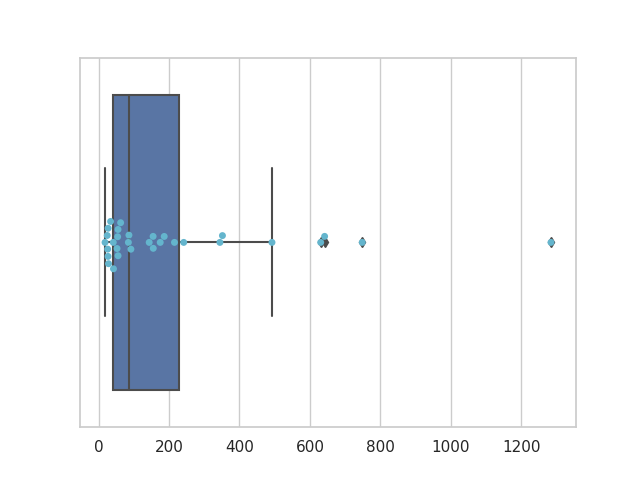
\includegraphics[scale=0.1]{src/main-matter/results/preliminary-testing/frequency/avg_pause_length_all}
%		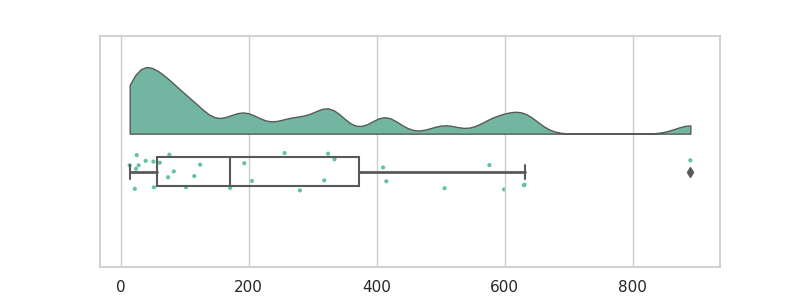
\includegraphics[scale=0.1]{src/main-matter/results/preliminary-testing/frequency/raincloud-pause-groups-num-all}
%		\caption{Where are the labels lmao?}
%		\label{default}
%	\end{center}
%\end{figure}

\subsection{Test 4: Dialogue - Audio File Comparison}
	\paragraph{Test Overview:} Testing calpy's capabilities given a 
	high fidelity audio file, recorded in ideal conditions, over an extended 
	period to determine the number of pauses that can be expected and how they compare to the Talkbank audio files. 
	Three ABC radio interviews were chosen to test the number of pauses that could be returned 
	given a high fidelity audio file recorded in ideal conditions and three of the best representative Talkbank files were chosen as comparison.
	This test aimed to provide a benchmark for pause counts to compare against the Talkbank files. 
	Files used were taken from the Australian Broadcasting Corporation (ABC).
%	\subsubsection{\underline{Test 6.1: High Quality - Ideal Conditions}}

%	\begin{enumerate}
%		\item low quality
%		\item high noise
%		\item poor conditions
%		\item ?? more ??
%	\end{enumerate}
%
%	This means the results can be highly susceptible to wrong or unusable results. 


%	\paragraph{File:} Files used were taken from the Australian Broadcasting Corporation (ABC)
%	\paragraph{Output:} Pause data in tables and figures showing how results compared to others visually
%	\paragraph{Result:} This showed pauses can be expected to be delivered anywhere from 1.44 to 1.76 pauses per second. 




%\paragraph{File Data Source:} 
%\footnotesize{data/dialogue/interview/abc/radio/programs/conversations/aaj-2019-04-24} 
%%\\
%%\smallsize data/dialogue/interview/abc/radio/programs/conversations/aaj-2019-04-26 \\
%%\smallsize data/dialogue/interview/abc/radio/programs/conversations/aaj-2019-04-29
%					
%%\end{description}
%
%\begin{table}[h]
%\begin{tabular}
%	{
%	|p{1.8cm}| 
%	|p{1.5cm} 
%	|p{1.5cm} 
%	|p{1.3cm} 
%	|p{1.1cm} 
%	|p{1.4cm} 
%	|p{1.5cm} 
%	|p{1.4cm}|
%	}
%	\hline
%	\multicolumn{8}{|c|}{ABC - Conversations} \\%
%	\hline
%	{\small Audio File} & 
%	{\footnotesize Time taken (min:sec)} & 
%	{\footnotesize Binary Pause Array Length} & 
%	{\footnotesize Total Audio Pause} & 
%	{\footnotesize Total Sounding} & 
%	{\footnotesize Pause Proportion} & 
%	{\footnotesize Num. of Pauses} & 
%	{\footnotesize Avg. Pause Length} \\
%		\hline\hline
%		%\cellcolor[HTML]{A2A1A2} 
%		aaj-2019-04-24 & 53:11 & 31914 & 22154 & 9760 & 69.42\% & 4622 & 479ms \\
%		\hline
%		aaj-2019-04-26 & 51:39 & 30986 & 15949 & 15037 & 51.47\% & 5432 & 294ms \\
%		\hline
%		aaj-2019-04-29 & 52:01 & 31209 & 19401 & 11808 & 62.16\% & 5007 & 387ms \\
%		\hline
%\end{tabular}
%\label{tab:aaj}
%\caption{Table: Pauses of various high quality ABC radio podcasts. Pause count is in the thousands, pause proportion is approximately 50\%-70\% and the average pause length is close to the 100ms lower bound.}
%\end{table}


%
%\subsubsection{\underline{Test 6.2: Compressed Quality - Non Ideal Conditions}}
%
%\paragraph{File Data Source:} 
%\footnotesize{data/dialogue/conversations/media.talkbank.org/ca/CallFriend/eng-n}
%
%\begin{table}[h]
%	\begin{tabular}{ | p{1.8cm} | | p{1.5cm} | p{1.5cm} | p{1.3cm} | p{1.1cm} | p{1.4cm} | p{1.5cm} | p {1.4cm} |}
%		\hline
%		\multicolumn{8}{| c |}{CallFriend - English (Northern)} \\%
%		\hline
%		{\small Audio File} & {\footnotesize Audio Length (min:sec)} &  {\footnotesize Binary Pause Array Length} & 
%			{\footnotesize Total Audio Pause} & {\footnotesize Total Sounding} & {\footnotesize Pause Proportion} & 
%			{\footnotesize Num. of Pauses} & {\footnotesize Avg. Pause Length} \\
%		\hline\hline
%		4175 & 30:00 & 17999 & 17149 & 850 & 95.28\% & 631 & 2718ms \\
%		\hline 
%		4708 & 30:00 & 17999 & 17365 & 634 & 96.48\% & 506 & 3432ms \\
%		\hline 
%%		\rowcolor{lightgray} 
%		4984 & 30:00 & 17999 & 16449 & 1,550 & 91.39\% & 890 & 1800ms \\
%		\hline
%\end{tabular}
%\label{tab:aaj}
%\caption{Table: Pauses of best representative talkbank audio files. Pause count is in the hundres, pause proportion is approximately 95\% of the audio and the average pause length is approximately 2600ms.}
%\end{table}

\begin{table}[ht]
	\begin{center}
	\begin{tabular}
		{ 
			|p{1.8cm}| |p
			{1.5cm}|p
			{1.5cm}|p
			{1.3cm}|p
			{1.1cm}|p
			{1.4cm}|p
			{1.5cm}|p 
			{1.4cm}|
		}
		\hline
		\multicolumn{8}{|c|}{Comparison Average of ABC, JJJ, Talkbank Comparison} \\%
		\hline
			{\small Audio File} & 
			{\footnotesize Audio Length (min:sec)} & 
			{\footnotesize Binary Pause Array Length} & 
			{\footnotesize Total Audio Pause} & 
			{\footnotesize Total Sounding} & 
			{\footnotesize Pause Proportion} & 
			{\footnotesize Num. of Pauses} & 
			{\footnotesize Avg. Pause Length} \\
		\hline
		\hline
		JJJ & 14:24 & 8578 & 6547 & 2031 & 75.18 \% & 737 & 974ms \\
		\hline
		JJJ & --:-- & 15,935 & 15,027 & 909 & 94.02 \% & 291 & 260ms \\
		\hline    
		%\rowcolor{lightgray} 
		Talkbank & 26:43 & 15825.3 & 15257.6 & 607.1 & 96.33 & 1194.55 & 4815.3ms \\
		\hline
	\end{tabular}
	\label{tab:1}
	\caption{Audio file comparison of the average ABC, JJJ and Talkbank results (outliers removed)} \\
	\end{center}
\end{table}
\clearpage

%\subsection{Test 5: Talkbank Waveform Analysis}
	\paragraph{Test:} 
	What the audio waveform looked like in comparison to the results that were returned to identify why talkbank results were so poor. 
	Possible reasons could be:
	\begin{itemize}
	\item{Noise affecting long pauses} 
	\item{poor digitisation} 
		\item interference,
		\item recording quality, 
%		\item someone might put the other on hold, 
		\item they might talk to quietly or too loudly,
		\item one may talk very loud and the other quiet
		\item maybe they talk far too close to the receiver and saturate the audio causing massive spikes in the waveform 
		\item the speakers voices (maybe high voices are better received and thus female audio files have better data
	\end{itemize}

This test involved looking at the audio files themselves and seeing how the waveform varied between files. A high level of variance was present between files, some files show extremely little waveform variance indicating low volume and some show extreme variance indicating flooding of noise. \\

	\subsubsection{callHome/eng/}
	
	\subparagraph{low variance files} 4683, 4689, 4694, 
	
	\subparagraph{high variance files} 4673, 4665, 4629, 4887, 4938, 5388
	
	\subparagraph{disgusting high variance} 4702, 4829, 4913, 4926, 4941, 5648, 6479, 6625

	\subparagraph{lots of spikes} 4677, 4838, 

	\subparagraph{lots of big consistent pauses} 4666, 4660, 
	
	\subparagraph{lots of small pauses} 4753
	
	\subparagraph{quiet} 4776, 4854, 
	
	\subparagraph{quiet low variance} 4910
	
	\subparagraph{high and low variance} 4807, 4808, 4824, 5208, 6282, 6313
	
	\subparagraph{consistent one speaker talking} 4844, 5046
	
	\subparagraph{put on hold} 4852
	
	\subparagraph{loud constant talking and quiet inconsistent} 4861
	
	\subparagraph{high and med variance} 4886, 
	
	\subparagraph{one quiet one constant talking} 4967

% \subsubsection{Exp7 - [2, 3, 4, 5, 6, 7, 8, 9, 10]}

 \begin{table}[htp]
	\scriptsize
	\begin{center}
	\begin{tabular}
		{ 
			|p{1.5cm}| |p
			{1.5cm}|p
			{.8cm}|p
			{.8cm}|p
			{.8cm}|p
			{.8cm}|
		}
		\hline
		\multicolumn{6}{|c|}{ABC - Radio - Program: Conversations} \\%
		\hline
			{\footnotesize Audio File} & 
			{\scriptsize Entropy Variance} & 
			{\scriptsize Mode} &
			{\scriptsize Mean} &
			{\scriptsize Median} & 
			{\scriptsize Range} \\
		\hline
		\hline

		%\cellcolor[HTML]{A2A1A2} 
		aaj-2019-03-15 & 41 - 47 & 44 & - & - & 6 \\
		\hline 
		aaj-2019-03-21 & 40 - 48 & 44 & - & - & 8 \\
		\hline 
		aaj-2019-03-27 & 38 - 42 & 40 & - & - & 4 \\
		\hline
		aaj-2019-04-11 & 37 - 43 & 40 & - & - & 6 \\
		\hline
		aaj-2019-04-24 & 37 - 43 & 40 & - & - & 6\\
		\hline
		aaj-2019-04-26 & 41 - 48 & 44 & - & - & 7 \\
		\hline
		aaj-2019-04-29 & 38 - 46 & 42 & - & - & 8 \\
		\hline
		aaj-2019-04-30 & - & - & - & - & - \\
		\hline
		aaj-2019-05-17 & - & - & - & - & - \\
		\hline
		aaj-2019-05-08 & - & - & - & - & - \\
		\hline
		aaj-2019-05-09 & - & - & - & - & - \\
		\hline
		\hline 
		Average & - & - & - & - & 6.43 \\
		\hline
		\hline

	\end{tabular}
	\label{tab:1}
	\caption{Pause usage of abc conversations audio files - preliminary statistical pause analysis 
	pertaining to middle aged participants with the results of SM.1 on each audio file with the total pauses
	 for that file and the pauses counted for each symbol} \\
	\end{center}
\end{table}


 \begin{table}[htp]
	\scriptsize
	\begin{center}
	\begin{tabular}
		{ 
			|p{1.5cm}| |p
			{1.5cm}|p
			{.8cm}|p
			{.8cm}|p
			{.8cm}|p
			{.8cm}|
		}
		\hline
		\multicolumn{6}{|c|}{ABC - Radio - Program: Mornings} \\%
		\hline
			{\footnotesize Audio File} & 
			{\scriptsize Entropy Variance} & 
			{\scriptsize Mode} &
			{\scriptsize Mean} &
			{\scriptsize Median} & 
			{\scriptsize Range} \\
		\hline
		\hline

		%\cellcolor[HTML]{A2A1A2} 
		- & 38 - 42 & 40 & - & - & 4 \\
		\hline 
		-- & 37 - 41 & 39 & - & - & 4 \\
		\hline 
		--- & 37.5 - 41.5 & 39.5 & - & - & 4 \\
		\hline
		-- & 40 - 44 & 42 & - & - & 4 \\
		\hline
		-- & 37 - 42 & 39 & - & - & 5\\
		\hline
		--- & 38.5 - 41.5 & 40 & - & - & 3 \\
		\hline
		-- & 38 - 42 & 40 & - & - & 4 \\
		\hline
		---- & - & - & - & - & - \\
		\hline
		-- & - & - & - & - & - \\
		\hline
		-- & - & - & - & - & - \\
		\hline
		-- & - & - & - & - & - \\
		\hline
		\hline 
		Average & - & - & - & - & 4 \\
		\hline
		\hline

	\end{tabular}
	\label{tab:1}
	\caption{Pause usage of abc conversations audio files - preliminary statistical pause analysis 
	pertaining to middle aged participants with the results of SM.1 on each audio file with the total pauses
	 for that file and the pauses counted for each symbol} \\
	\end{center}
\end{table}




So what does high entropy mean, greater distributed use of the symbols? 

What does high variance mean then? Inconsistent use of pauses. Maybe it was the style of conversation? 

How is it higher variance? Are they hitting higher peaks? Lower troughs? 

What does it tell us about the groups? Maybe the longer length of conv allowed for different use of pauses (relaxed? does that account for the variance?)

This shows the variance tends to be greater for --- conversations, indicating the information theyre giving tends to move from high information to low more frequently whereas -- people tend to stick to a common entropy value more often.

Not only were the outlier points greater for conversations, but I think they tended to fluctuate more often between those points.








